%
%
%  This file is inserted in the file Segmentation.tex
%
%

\subsection{Overview}
\label{sec:AboutWatersheds}
\index{Watersheds|textbf}
\index{Watersheds!Overview}

Imagine water raining onto a landscape topology and flowing with gravity to
collect in low basins.  The size of those basins will grow with increasing
amounts of precipitation until they spill into one another, causing small
basins to merge together into larger basins.  Analogously, watershed
segmentation classifies pixels into regions using gradient descent on image
features and analysis of weak points along region boundaries. Regions
(catchment basins) are formed by using local geometric structure to associate
points in the image domain with local extrema in some feature measurement such
as curvature or gradient magnitude.  This technique is less sensitive to
user-defined thresholds than classic region-growing methods, and may be better
suited for fusing different types of features from different data sets.  The
watersheds technique is also more flexible in that it does not produce a single
image segmentation, but, rather, a hierarchy of segmentations from which a
single region or set of regions can be extracted a-priori, using a threshold,
or interactively with the help of a graphical user interface
\cite{Yoo1992,Yoo1991}.

The strategy of watershed segmentation is to treat an image $f$ as a height
function, i.e.  the surface formed by graphing $f$ as a function of its
independent parameters, $\vec{x} \in U$.  The image $f$ is often not the
original input data, but is derived from that data through some filtering,
graded (or fuzzy) feature extraction, or fusion of feature maps from different
sources.  The assumption is that higher values of $f$ (or $-f$) indicate the
presence of boundaries in the original data.  Watersheds may therefore be
considered as a final or intermediate step in a hybrid segmentation method,
where the initial segmentation is the generation of the edge feature map.

Gradient descent associates regions with local minima of $f$ (clearly interior
points) using the watersheds of the graph of $f$, as in
Figure~\ref{fig:segment}.
\begin{figure}
\centering
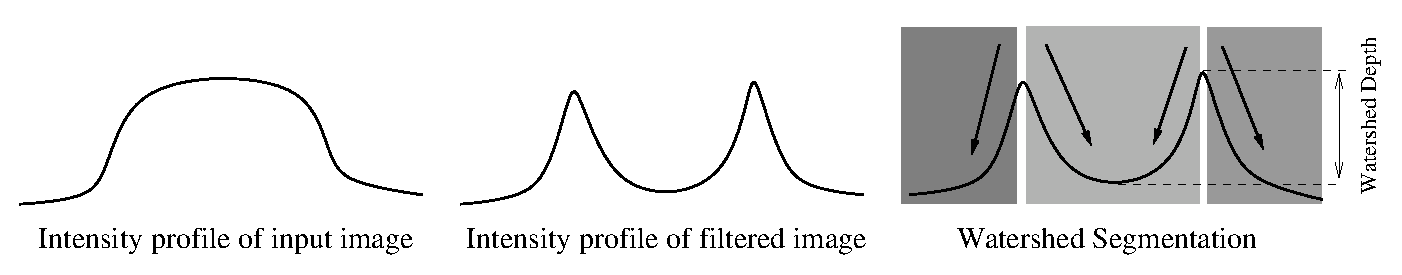
\includegraphics[width=0.9\textwidth]{WatershedCatchmentBasins.eps}
\caption{A fuzzy-valued boundary map, from an image or set of images, 
is segmented using local minima and catchment basins.}
\protect\label{fig:segment}
\end{figure}
That is, a segment consists of all points in $U$ whose paths of steepest
descent on the graph of $f$ terminate at the same minimum in $f$.  Thus, there
are as many segments in an image as there are minima in $f$.  The segment
boundaries are ``ridges'' \cite{Koenderink1979,Koenderink1993,Eberly1996} in
the graph of $f$.  In the 1D case ($U \subset \Re$) the watershed boundaries
are the local maxima of $f$, and the results of the watershed segmentation is
trivial.  For higher-dimensional image domains, the watershed boundaries are
not simply local phenomenon, they depend on the shape of the entire watershed.

The drawback of watershed segmentation is that it produces a region for each
local minimum, which is often, in practice, too many regions---an over
segmentation.  To alleviate this, we can establish a minimum watershed depth.
The watershed depth is the difference in height between the watershed minimum
and the lowest boundary point.  That is, the maximum depth of water a region
could hold without flowing into any of its neighbors.  Thus, a watershed
segmentation algorithm can sequentially combine watersheds whose depths fall
below the minimum until all of the watersheds are of sufficient depth.  This
depth measurement can be combined with other saliency measurements, such as
size.  The result is a segmentation containing regions whose boundaries and
size are significant.  Because the merging process is sequential, it produces a
hierarchy of regions, as shown in Figure~\ref{fig:watersheds}.
\begin{figure}
\centering
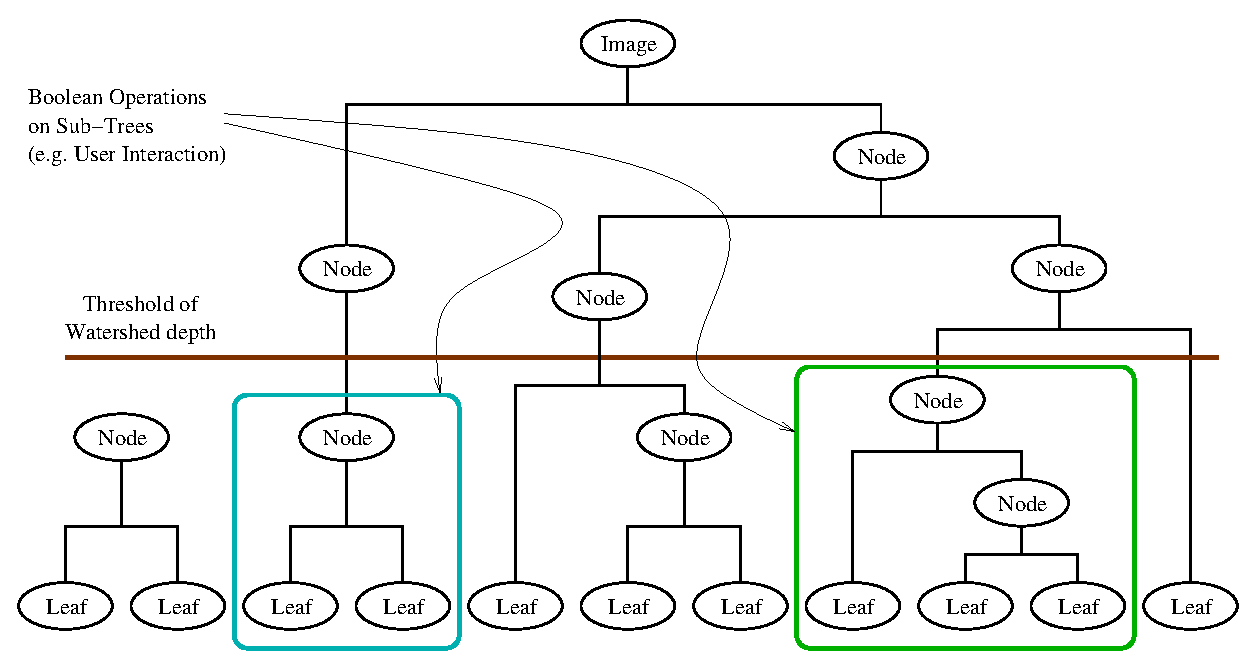
\includegraphics[width=0.9\textwidth]{WatershedsHierarchy.eps}
\caption{A watershed segmentation combined with a saliency measure 
(such as depth) produces a hierarchy of regions.  Structures can be 
derived from images by either thresholding the saliency measure or 
combining subtrees within the hierarchy}
\protect\label{fig:watersheds}
\end{figure}
Previous work has shown the benefit of a user-assisted approach, which provides
a graphical interface to this hierarchy so that a technician can quickly move
from the small regions that lie within a area of interest to the union of
regions that correspond to the anatomical structure \cite{Yoo1991}.

There are two different algorithms commonly used to implement watersheds,
top-down and bottom-up.  The top-down, gradient descent strategy was chosen for
ITK because we want to consider the output of multi-scale differential
operators, and the $f$ in question will therefore have floating point
values. The bottom-up strategy starts with seeds at the local minima in the
image and grows regions outward and upward at discrete intensity levels
(equivalent to a sequence of morphological operations and sometimes called {\em
morphological watersheds} \cite{Serra1982}.) This limits the accuracy by
enforcing a set of discrete gray levels on the image.

Figures~\ref{fig:WatershedColorSegmentation1}--~\ref{fig:WatershedColorSegmentation3}
show the results of segmenting the color image from
Figure~\ref{fig:WatershedColorInput}(a).  These results are obtained by
applying the watershed algorithm to the root-sum-of-squares gradient magnitude
shown in Figure~\ref{fig:WatershedColorInput}(b).  By changing the threshold on
the minimum watershed depth, we can obtain different degrees of segmentation.
No one segmentation is ``perfect''; at one level the spinal cord is segmented
into various tracts, while at another level it comes together to form a single
structure.  Smaller regions can be expanded into larger regions by either
changing the depth threshold or combining them under some user direction.

\begin{figure}
\centering
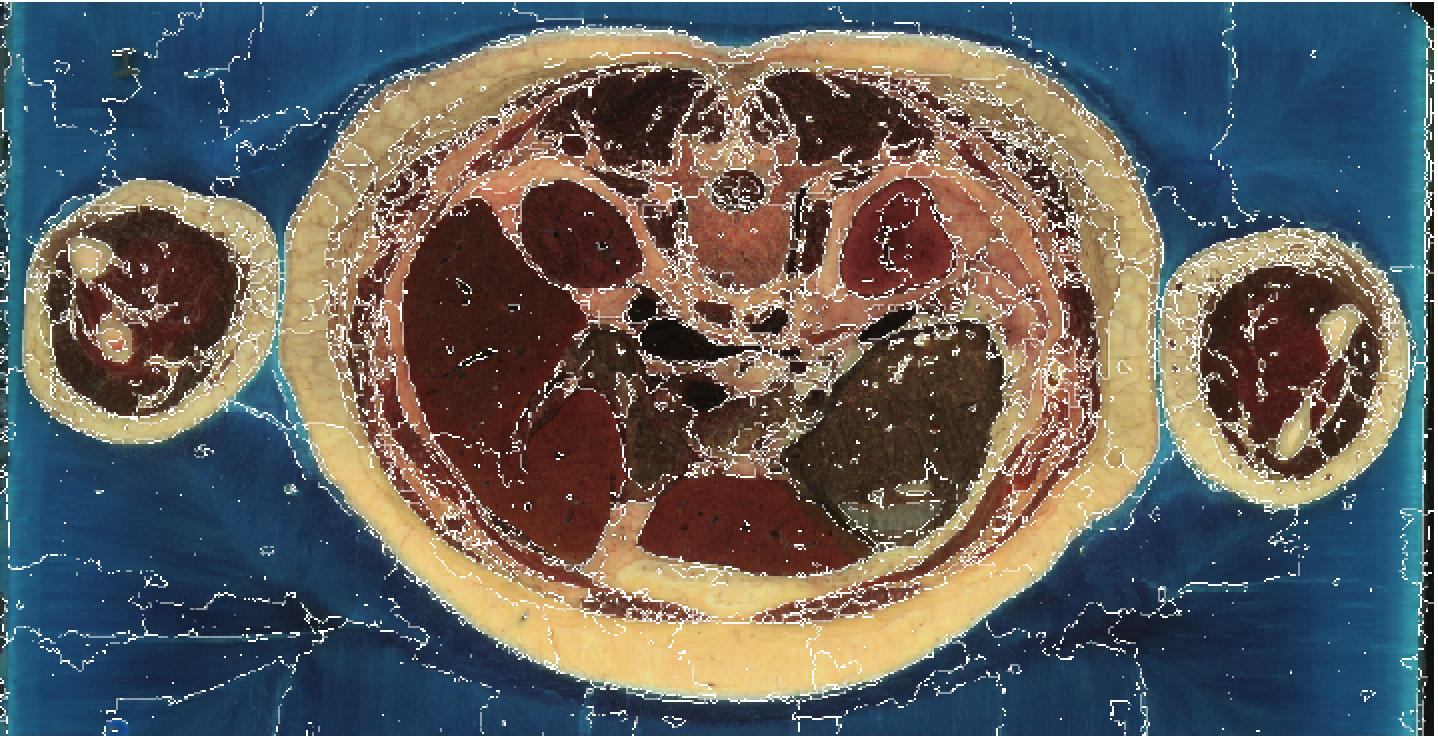
\includegraphics[width=0.9\textwidth]{WatershedColorEdges.eps}
\caption{
A segmentation (white lines are segment boundaries) based on 
the gradient magnitude of a color image that has been processed with 
vector-valued anisotropic diffusion.}
\protect\label{fig:WatershedColorSegmentation1}
\end{figure}
\begin{figure}
\centering
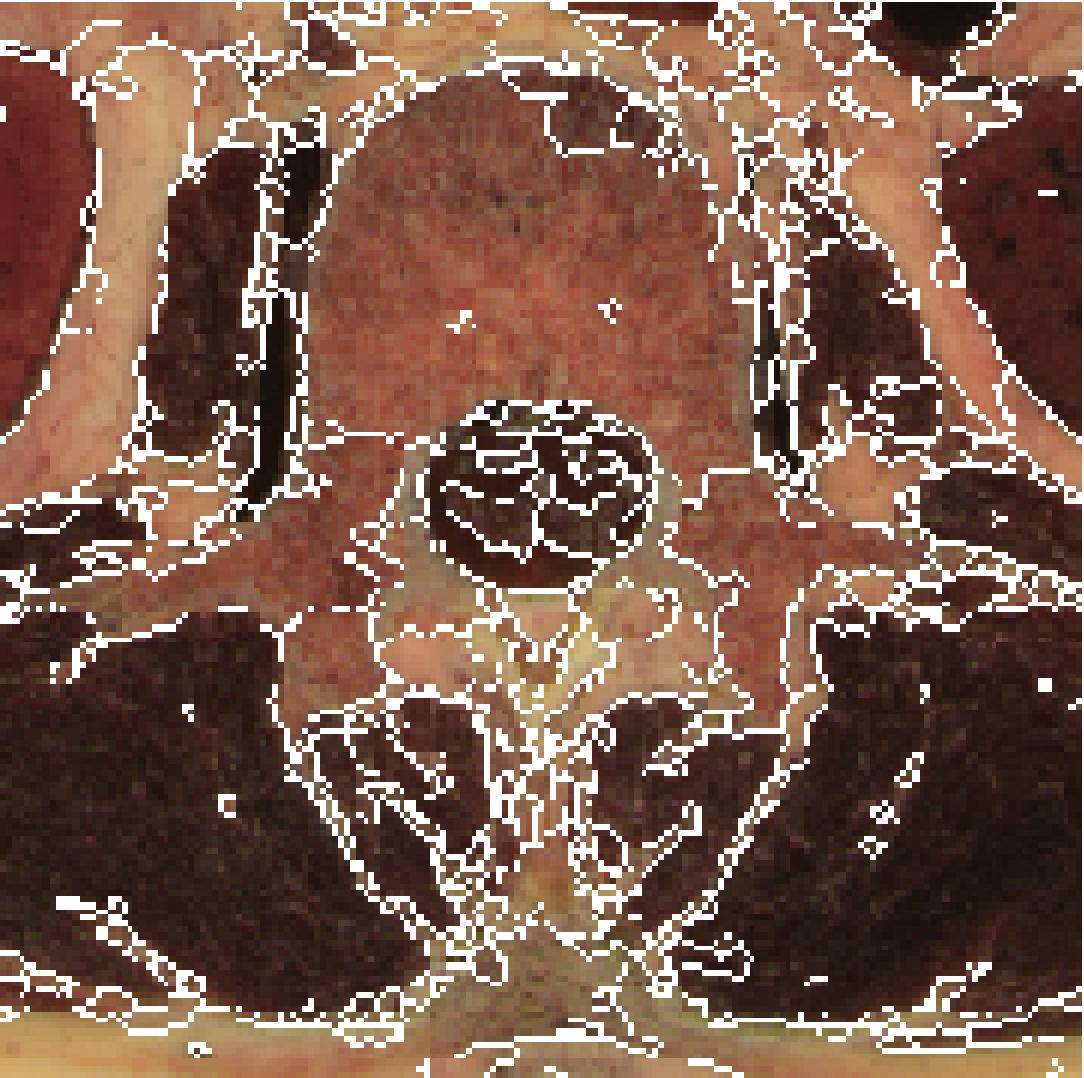
\includegraphics[width=0.4\textwidth]{WatershedSpine1.eps}
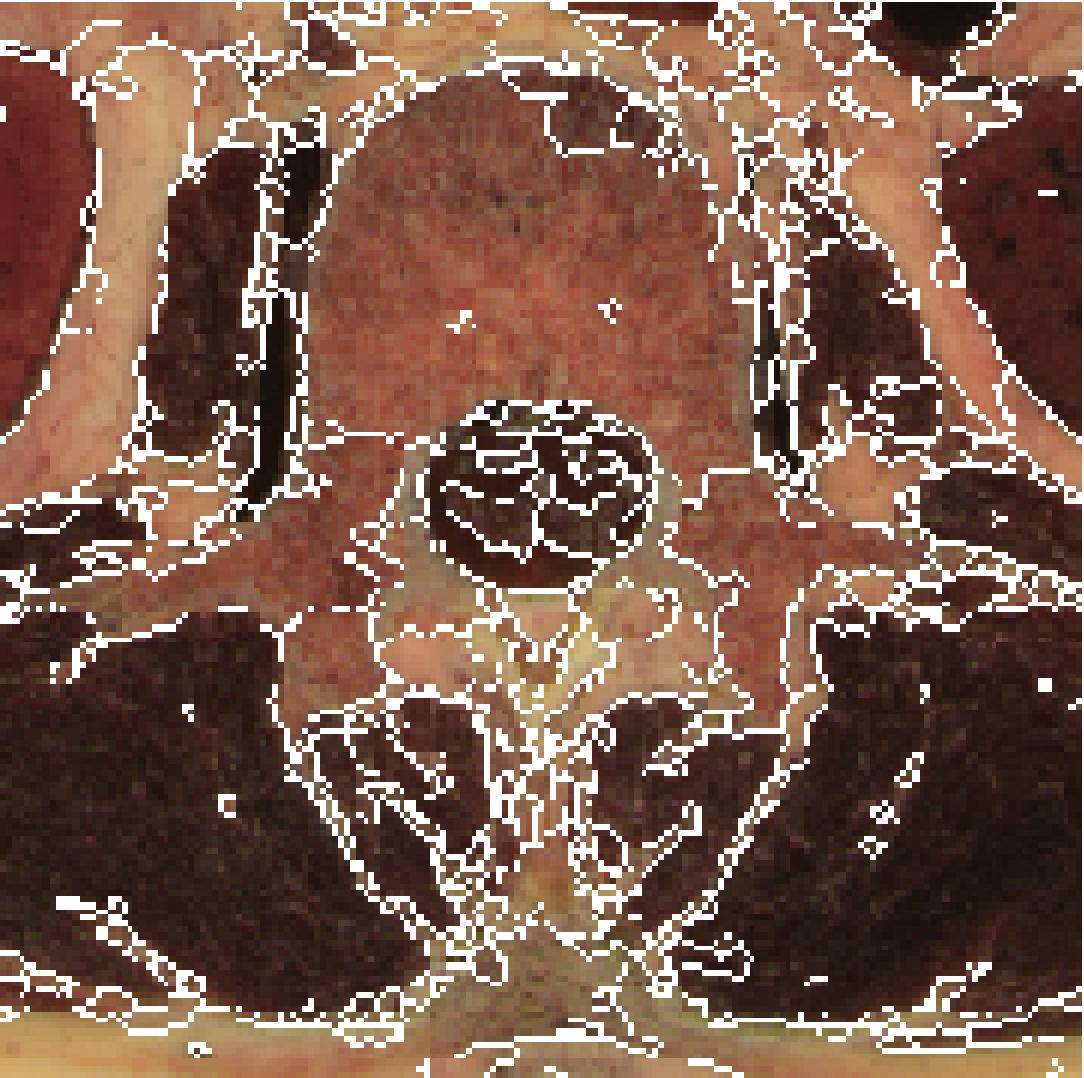
\includegraphics[width=0.4\textwidth]{WatershedSpine1.eps}
\caption{
Insets from the segmentation of the color image shown in 
Figure~\protect\ref{fig:WatershedColorSegmentation1} at two different levels of 
watershed depth.  Top) A lower threshold partitions the spinal cord
into several distinct tracts.  Bottom) At a higher threshold the 
vertebrae becomes a single segment and the parts of the 
spinal cord merge.
}
\protect\label{fig:WatershedColorSegmentation2}
\end{figure}

\begin{figure}
\centering
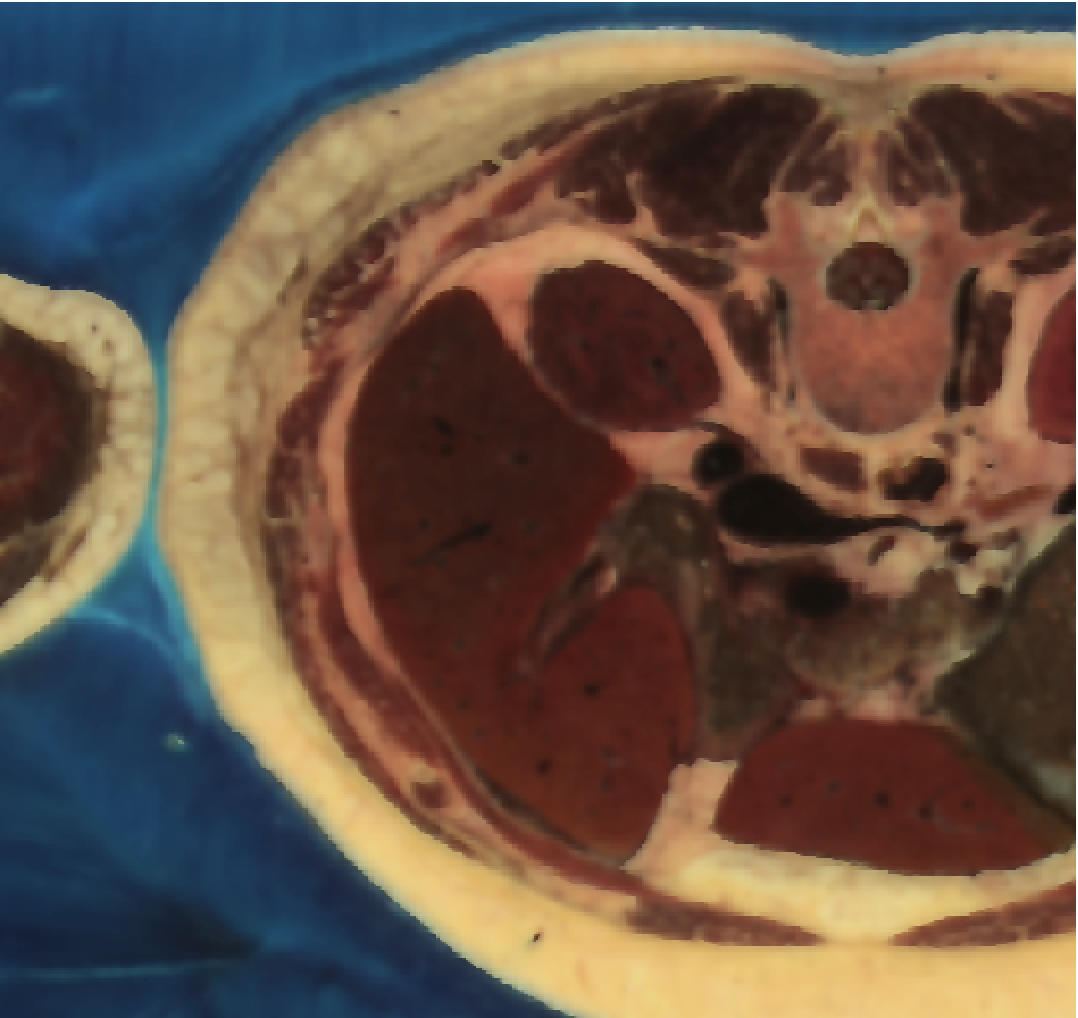
\includegraphics[width=0.4\textwidth]{WatershedColorInput.eps}
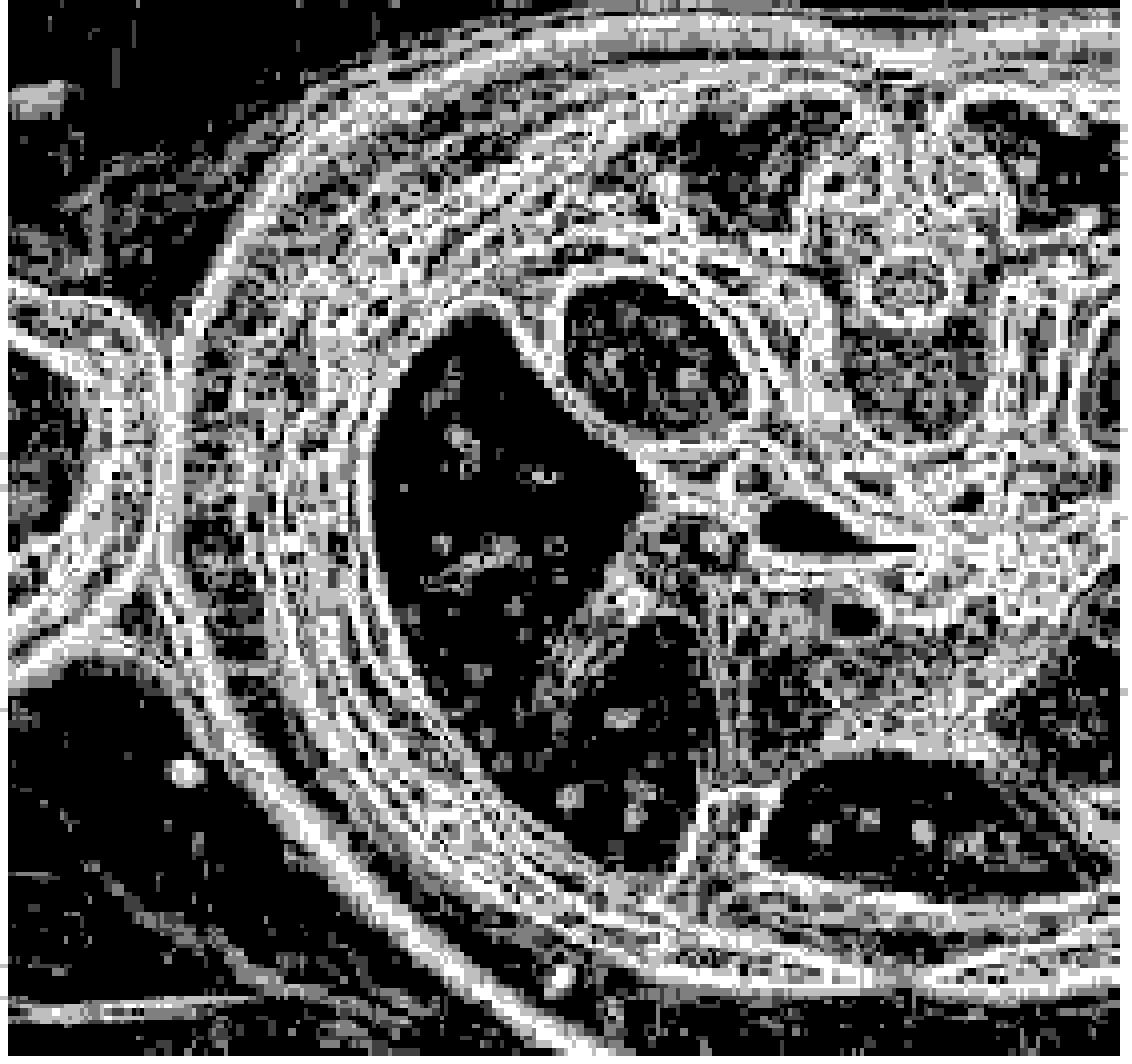
\includegraphics[width=0.4\textwidth]{WatershedColorGradientMagnitude.eps}
\caption{
Inputs for the segmentation presented in \ref{fig:WatershedColorSegmentation3}.
Left) Cryogenic data set after smoothing with anisotropic diffusion.  Right)
Squared magnitude of gradients on every color channel.}
\protect\label{fig:WatershedColorInput}
\end{figure}

\begin{figure}
\centering
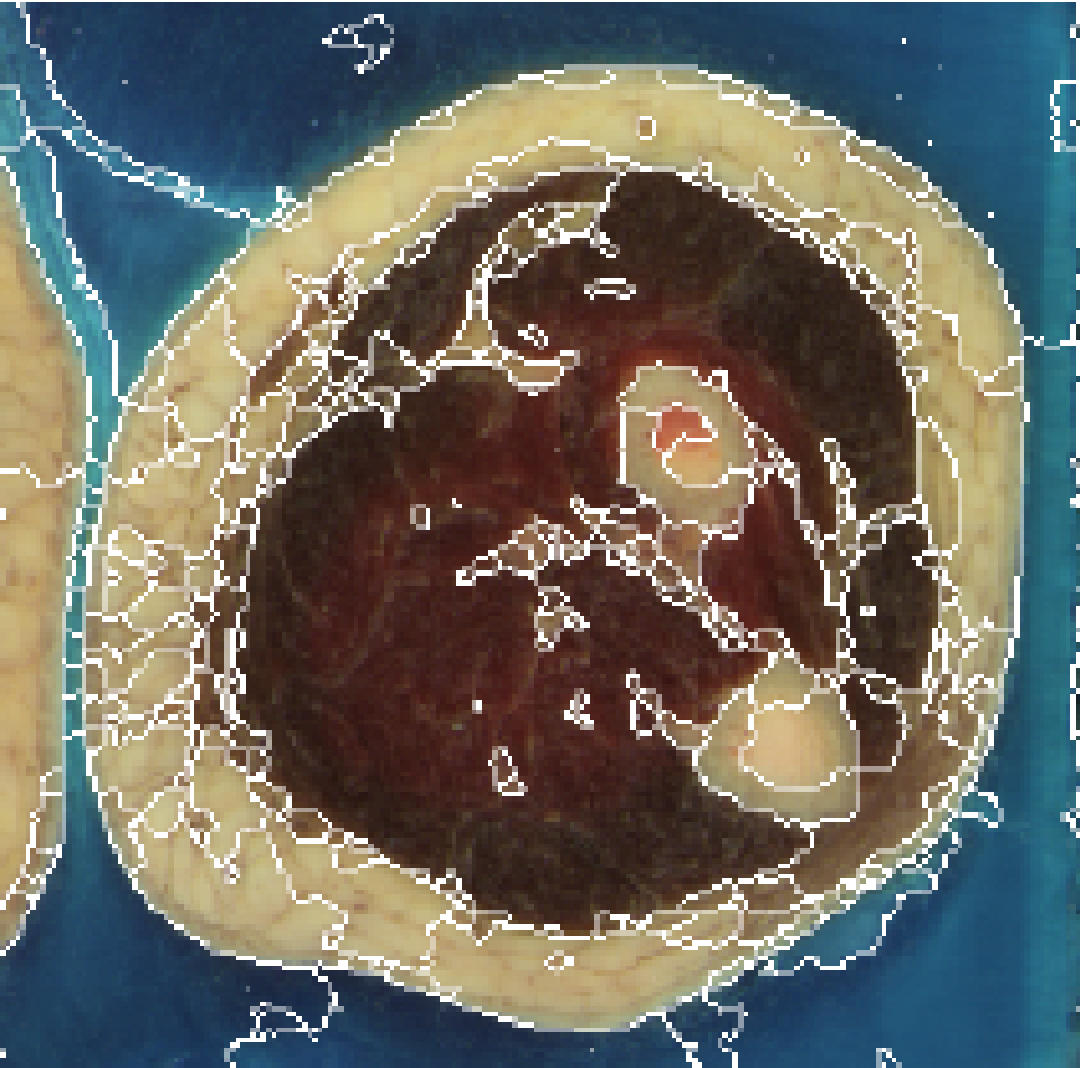
\includegraphics[width=0.4\textwidth]{WatershedArm1.eps}
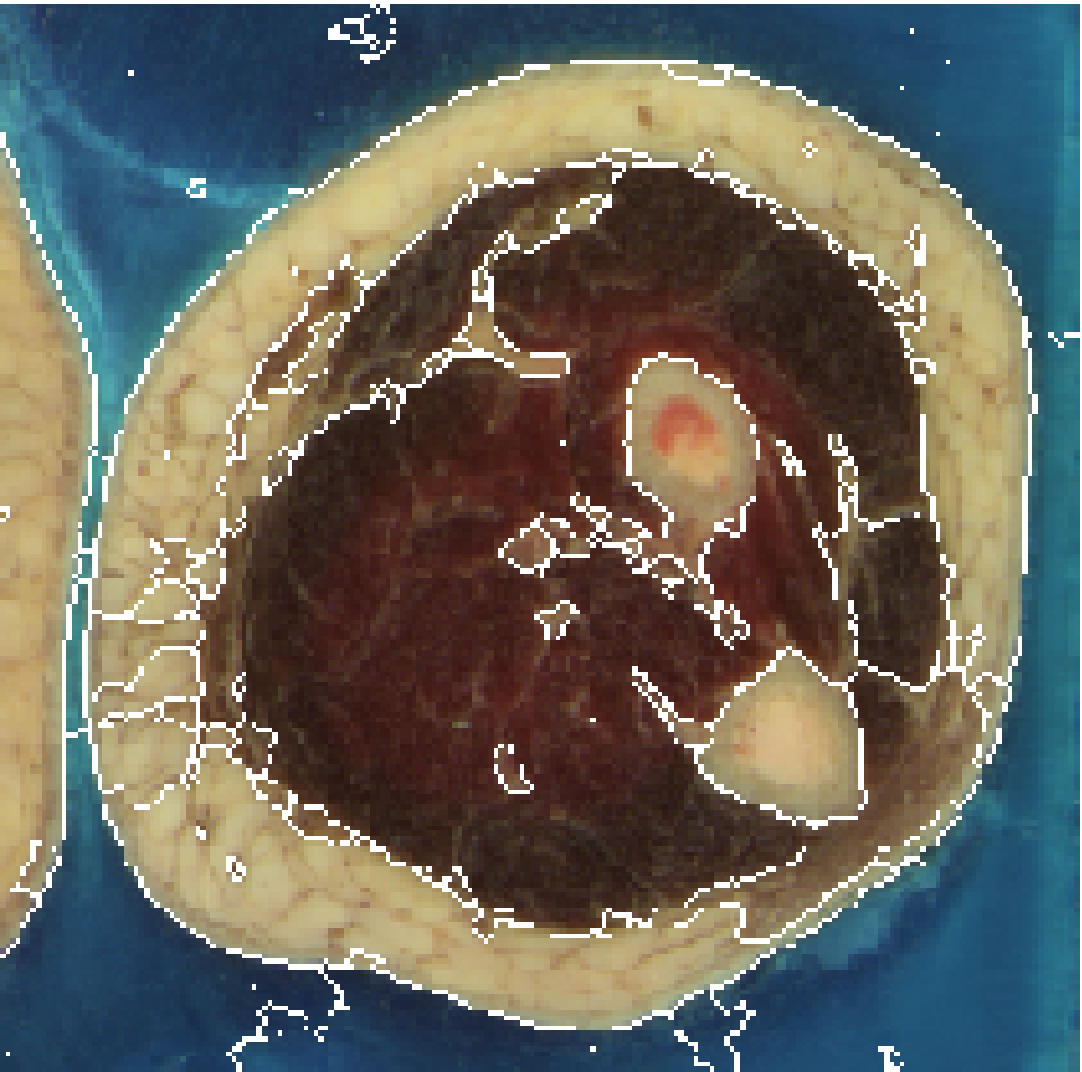
\includegraphics[width=0.4\textwidth]{WatershedArm2.eps}
\caption{
Insets from the segmentation of the color image shown in 
Figure~\protect\ref{fig:WatershedColorSegmentation1} at two different levels of 
watershed depth.  Top) The fat around the arm consists of many 
distinct regions.  Bottom) At a higher threshold the 
fat becomes a single segment as do the bones.
}
\protect\label{fig:WatershedColorSegmentation3}
\end{figure}
\subsection{Watershed Segmentation in Insight}
\label{sec:ImplementationWatersheds}
\index{Watersheds!Segmentation}

\begin{figure}
\centering
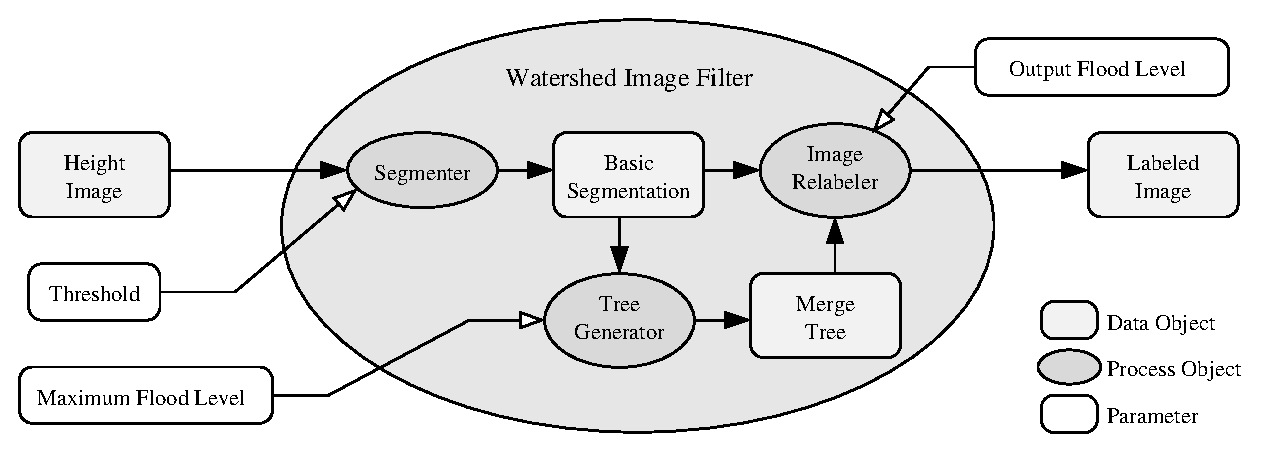
\includegraphics[width=0.9\textwidth]{WatershedImageFilter.eps}
\caption{The construction of the Insight watersheds filter.}
\protect\label{fig:constructionWatersheds}
\end{figure}

Figure~\ref{fig:constructionWatersheds} shows how the Insight image-to-image
watersheds filter is constructed.  The filter is actually a collection of
smaller filters which modularize the several steps of the algorithm in a
mini-pipeline.  The segmenter object creates the initial segmentation via
steepest descent from each pixel to local minima. Shallow background regions
are removed (flattened) before segmentation using a simple minimum value
threshold (this helps to minimize oversegmentation of the image).  The initial
segmentation is passed to a second sub-filter which generates a hierarchy of
basins to a user-specified maximum watershed depth.  The relabeler object at
the end of the mini-pipeline uses the hierarchy and the initial segmentation to
produce an output image at any scale {\em below} the user-specified maximum.
Data objects are cached in the mini-pipeline so that changing watershed depths
only requires a (fast) relabeling of the basic segmentation.  The three
parameters which control the filter are shown in the
Figure~\ref{fig:constructionWatersheds} connected to their relevant processing
stage.

\subsection{Using the Insight Watershed Filter}
\label{sec:UsingWatersheds}
\index{Watersheds!ImageFilter}
The care with which the input to the watershed filter is prepared will greatly
affect the quality of your result.  As noted in
Section~\ref{sec:AboutWatersheds}, the height function used as input should be
created such that higher positive values correspond to object boundaries.  A
suitable height function for many applications can be generated as the gradient
magnitude of the image to be segmented.  Typically, the best results are
obtained by preprocessing the original image with an edge-preserving diffusion
such as one of the anisotropic diffusion filters, or with the bilateral image
filter.  The height image input to itk::WatershedImageFilter should be of a
scalar, floating point type.

Tuning the filter parameters for any particular application is a process of
trial and error.  The {\em threshold} parameter can be used to great effect in
controlling oversegmentation of the image.  Raising the threshold will
generally reduce computation time and produce output with fewer and larger
regions.  The trick in tuning paramters is to consider the scale level of the
objects you are trying to segment.  The best time/quality trade-off will be
achieved when the image is smoothed and thresholded to eliminate features just
below the desired scale.

Most of the computational complexity of the ITK algorithm lies in generating
the hierarchy. Processing times for this stage are non-linear with respect to
the number of catchment basins in the basic segmentation.  This means that the
amount of information contained in an image is more significant than the number
of pixels in the image when predicting execution times.  A very large, but very
flat input may process in a much shorter time than a very small, but very
detailed input.  In practice, however, very large volumes do tend to increase
merge times exponentially because scale of the targeted objects does not
necessarily change proportional to increased resolution of the image.  When
going from lower to higher dimensionality, increased interconnectivity of
catchment basins can also result in non-linear increases in processing time.

\subsection{Interpreting the Results}
\label{sec:VisualizingWatersheds}
\index{Watersheds!Visualization}
In order to interpret the output of the Insight watersheds algorithm, it is
important to understand what the output represents and how it is formatted. The
itk::WatershedImageFilter produces an image of unsigned long integers.  Each
integer number is a label for a unique segmented region (catchment basin) from
the original input.  The output is the same size and dimensionality of the
input.

Because the segmented image may have potentially many thousands of labels, some
care must be taken when visualizing the data or information may be lost.  One
effective way to visualize the output is to map the integer labels into
distinct RGB colors.  Because labels close in value tend to also be close
spatially in the image, it is helpful to spread sequential label values far
apart in the RGB range.  A hashing scheme that puts more weight on the
least-significant integer bits is a good way to accomplish this.
Figure~\ref{fig:colorVisWatersheds} shows a slice taken from a segmentation of
a section of abdomen from the Visible Female Cryosection data.  The unsigned
long label values of the output have been hashed into RGB colors.

\begin{figure}
\centering
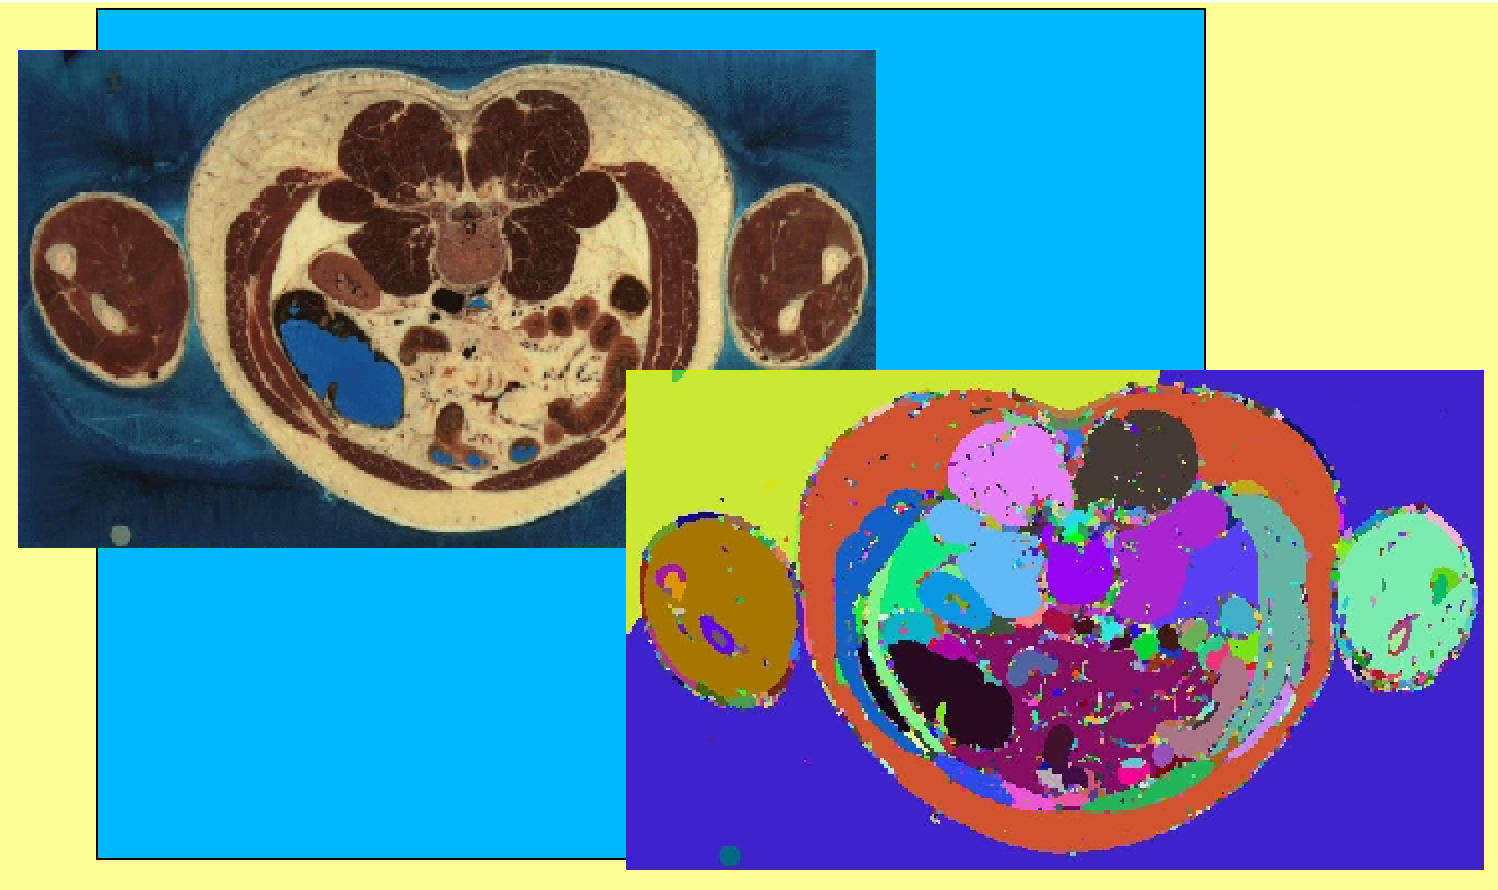
\includegraphics[width=.95\textwidth]{WatershedAbdomenSegmentation.eps}
\caption{A slice from a segmentation of Visible Female cryosection data.
The original is shown at the left and the segmented image is shown to the
right. Colored regions in the segmented image correspond to structures in the
original data. }
\protect\label{fig:colorVisWatersheds}
\end{figure}

For volumetric data, it is often interesting to create a surface rendering of
one or more regions in the output.  This can be done by thresholding the
region(s) of interest from the output image and exporting the result to a
visualization package capable of isosurface rendering.  Thresholding can be
done either by explicit manipulation of the image values through an ITK image
iterator, or using one of the several Insight image thresholding filters.

Figure~\ref{fig:surfaceRenderingWatersheds} is a surface rendering of the right
eye, the optic nerve and chiasm, the lens of the eye, and the right lateral
rectus muscle.  A slice from the original Visible Female head and neck
cryosection data from which the segmentations were created is shown at the
left.  This image was created as described above by thresholding isovalues in a
watershed segmentation output and then rendered using third-party visualization
software.

\begin{figure}
\centering
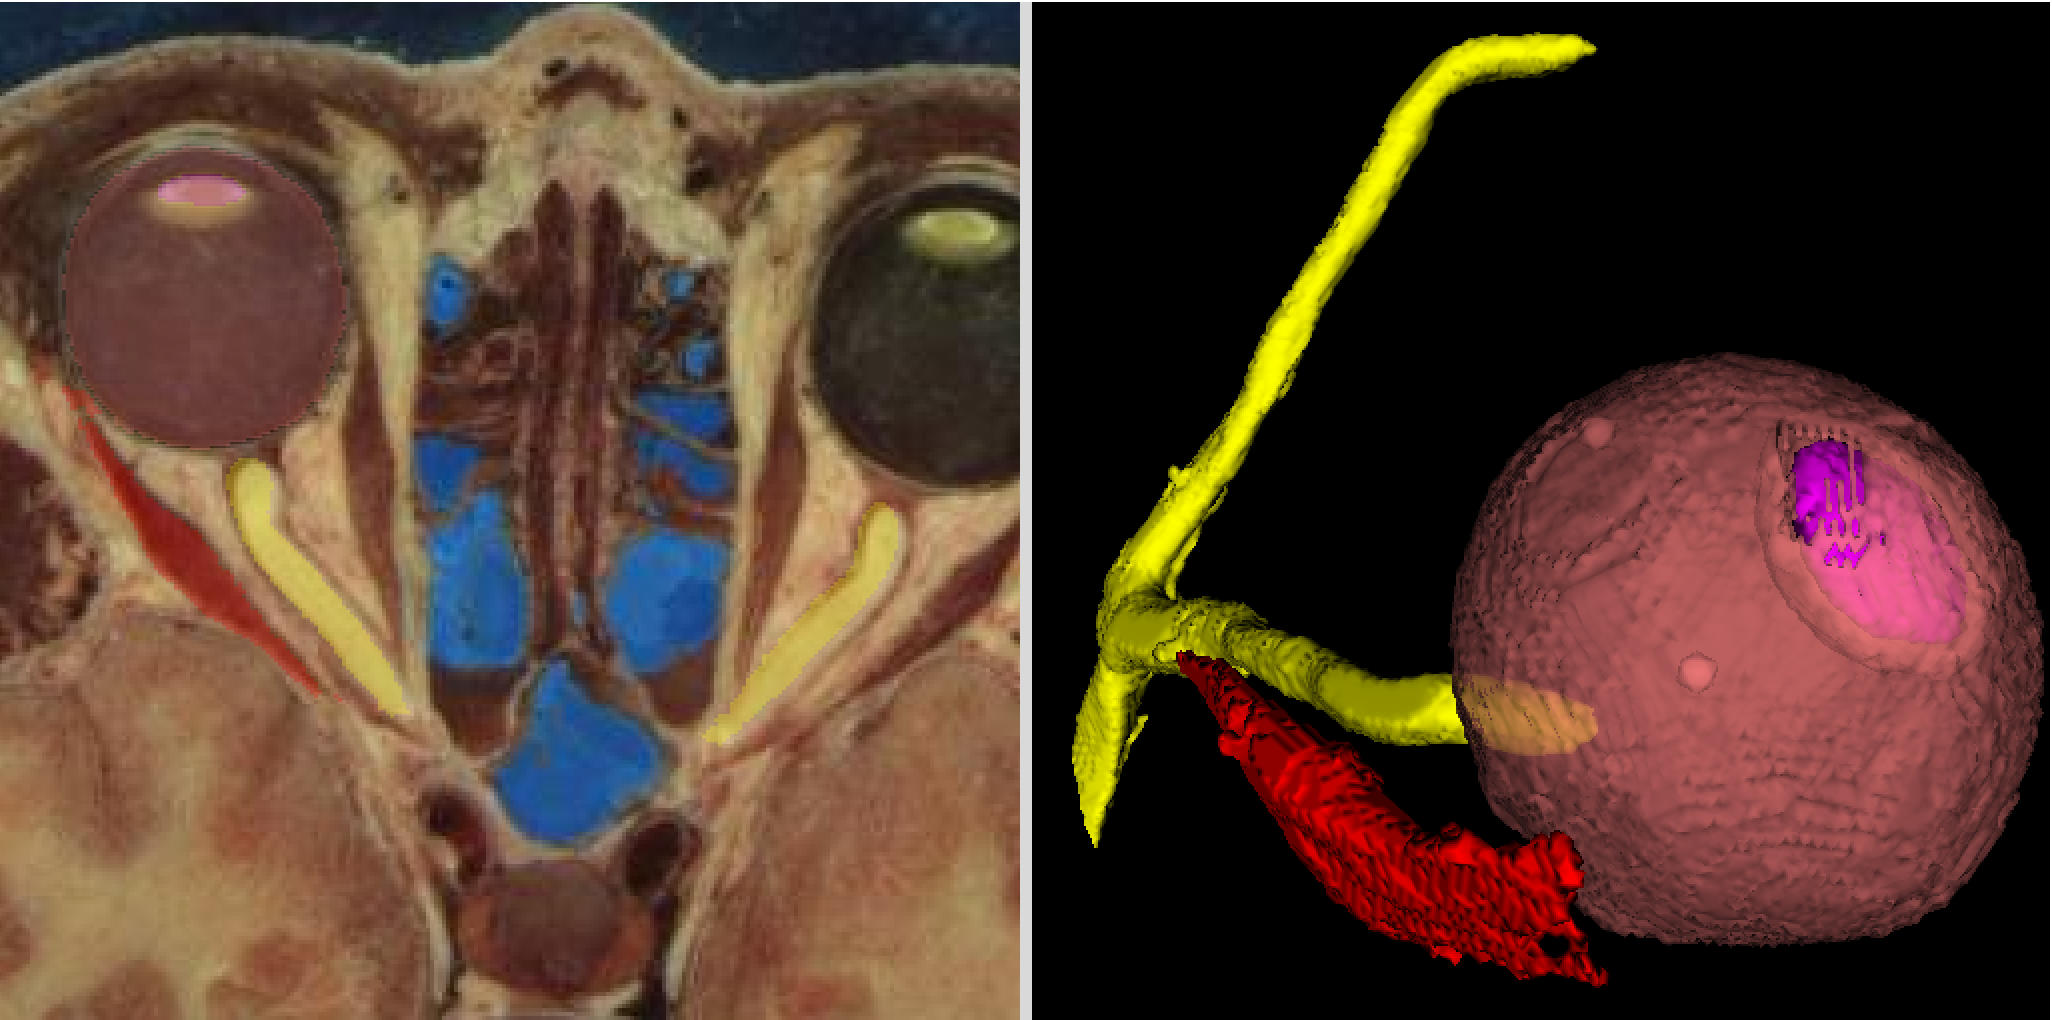
\includegraphics[width=0.95\textwidth]{WatershedRendering.eps}
\caption{A surface rendering (right) of four anatomical structures in the Visible
Female head and neck. A slice of the data from which the segmentation was
created is shown at the left.  The right and left optic nerves and chiasm are
shown in yellow.  The right eye is in transparent purple.  The lens is dark
purple.  The structure in red is the lateral rectus muscle.}
\protect\label{fig:surfaceRenderingWatersheds}
\end{figure}

